\section{Results}
\label{sec:results}

This section reports evaluation of \macaron{} across Personal Intelligence, agent, coding, and GenUI benchmarks. We compare \venti{} with Opus 4.8~\citep{anthropic_opus48_2026}, GPT-5.5~\citep{openai_gpt55_2026}, Gemini 3.1 Pro~\citep{gemini31pro_2026}, GLM-5.2~\citep{glm52_2026,glm5_2026}, Qwen 3.7 Max~\citep{qwen37max_2026}, and Minimax M3~\citep{minimax_m3_2026}. Table~\ref{tab:eval_results} reports the benchmark point estimates with provenance markers. Within each benchmark, unstarred values use the same task set and benchmark-specific evaluation protocol; starred values are imported public results included for context.

\subsection{Setup}
\label{sec:results_setup}

\paragraph{Models under test.}
\venti{} is the 748B-labeled release built from a frozen 744B GLM-5.2 base~\citep{glm52_2026,glm5_2026} and four LoRA specialists~\citep{lora2022}. The public adapter headers contain 7.688B stored values per specialist, so the release label is not used as a literal residency count. \tall{} is the 50B-labeled configuration built on Qwen3.6-35B-A3B~\citep{qwen36_2026,qwen3_2025}; its four public adapter headers contain 3.776B values each, giving approximately 50.1B on a nominal-base-plus-adapter count. Both are served through the \molshort{} harness described in Section~\ref{sec:mol}~\citep{mol_harness2026}. The separately merged \codingventi{} checkpoint is excluded from all tables and claims in this section.

\paragraph{Baselines.}
The comparison set comprises the six models listed above. All locally evaluated systems follow the benchmark-specific protocol documented in Appendix~\ref{app:eval_protocols}. The SWE and terminal evaluations use the Claude Code agent scaffold rather than the production \molshort{} harness, while UI4A-Bench baselines use adapter-free \uifora{}. Cells marked~\(\ast\) are imported from a public leaderboard or model report and serve as contextual reference points.

\paragraph{Benchmarks and metrics.}
Personal Intelligence comprises \chatbench{} (Section~\ref{sec:chatbench}) and \livingbench{} (Section~\ref{sec:livingbench})~\citep{macaron_v1_blog2026,macaron_v1_preview2026}. The agent group contains VitaBench~\citep{vitabench2026}, VitaBench2~\citep{chen2026vitabench2}, $\tau^3$-Bench, PinchBench~\citep{pinchbench2026}, and ClawGym. Coding contains SWE-Verified~\citep{jimenez2024swebench}, DeepSWE~\citep{deepswe2026}, and SWE Atlas QnA~\citep{sweatlas2026}; TerminalBench 2.1~\citep{terminalbench2026} measures terminal operation; and UI4A-Bench~\citep{ui4abench2026} measures generative UI. Appendix~\ref{app:eval_protocols} gives the metric, case-count, judge, retry, and aggregation details available for these twelve benchmark rows.

\subsection{Main Results}
\label{sec:results_main}

Table~\ref{tab:eval_results} reports \venti{} and six closed and open-weight baselines across twelve benchmark rows. It deliberately omits winner highlighting because the rows use different estimands and some cells are imported. Table~\ref{tab:eval_tall} separately gives a matched, within-row comparison of the 50B-labeled \tall{} system with its 35B-A3B base on the seven benchmarks available for both systems.

\begin{table}[!t]
  \centering
  \caption{Row-specific benchmark point estimates for \venti{} and six comparison models (higher is better; displayed on a 0--100 scale). Unstarred values within a row use the same benchmark-specific protocol; \(\ast\) marks an imported public value. Metrics and protocols differ across rows, so the table does not define an aggregate model ranking.}
  \label{tab:eval_results}
  \footnotesize
  \setlength{\tabcolsep}{4.25pt}
  \begin{tabular}{lccccccc}
    \toprule
    Benchmark & \venti{} & GLM-5.2 & GPT-5.5 & Opus 4.8 & Gemini 3.1 & Qwen 3.7 & Minimax M3 \\
    \midrule
    \multicolumn{8}{l}{\emph{Personal Intelligence}} \\
    ChatBench          & 58.3 & 54.5 & 55.5 & 52.8 & 52.0 & 52.5 & 49.1 \\
    LivingBench        & 64.0 & 60.5 & 61.9 & 63.8 & 52.1 & 56.1 & 57.1 \\
    \midrule
    \multicolumn{8}{l}{\emph{Agent}} \\
    VitaBench          & 60.0 & 55.8 & 55.8 & 56.5 & 55.2 & 61.2 & 56.8 \\
    VitaBench2         & 46.0 & 43.1 & 47.4 & 46.3 & 50.2 & 47.6 & 39.4 \\
    $\tau^3$-Bench     & 69.3 & 69.1 & 61.1 & 67.7 & 67.1$^{\ast}$ & 63.0 & 61.2 \\
    PinchBench         & 94.0 & 88.1 & 89.0\(^{\ast}\) & 91.8\(^{\ast}\) & 82.9\(^{\ast}\) & 93.4\(^{\ast}\) & 86.1 \\
    ClawGym            & 77.7 & 74.6 & 82.5 & 80.5 & 77.5 & 75.7 & 76.2 \\
    \midrule
    \multicolumn{8}{l}{\emph{Coding and terminal}} \\
    SWE-Verified       & 85.6 & 80.4 & 82.9\(^{\ast}\) & 88.6\(^{\ast}\) & 80.6\(^{\ast}\) & 80.4\(^{\ast}\) & 80.5\(^{\ast}\) \\
    TerminalBench 2.1  & 87.6 & 82.7\(^{\ast}\) & 83.4\(^{\ast}\) & 78.9\(^{\ast}\) & 70.7\(^{\ast}\) & 73.5\(^{\ast}\) & 66.0\(^{\ast}\) \\
    DeepSWE            & 58.4 & 54.9\(^{\ast}\) & 70.0\(^{\ast}\) & 58.0\(^{\ast}\) & 10.0\(^{\ast}\) & 18.0\(^{\ast}\) & 20.0\(^{\ast}\) \\
    SWE Atlas QnA      & 49.5 & 48.9\(^{\ast}\) & 45.4\(^{\ast}\) & 57.3\(^{\ast}\) & 13.5\(^{\ast}\) & 22.6 & 37.9 \\
    \midrule
    \multicolumn{8}{l}{\emph{GenUI (Final Score)}} \\
    UI4A-Bench         & 87.8 & 67.1 & 72.1 & 75.9 & 60.3 & 62.5 & 63.0 \\
    \bottomrule
  \end{tabular}
\end{table}

\begin{table}[!t]
  \centering
  \caption{Comparison of \tall{} (50B release label; approximately 50.1B by nominal base plus public adapter tensors) with its Qwen3.6 35B-A3B base on the seven benchmarks evaluated for both systems (higher is better; normalized to 0--100). Both systems use the same protocol within each row. This is an end-to-end system comparison rather than a parameter-matched component ablation; bold marks the larger score.}
  \label{tab:eval_tall}
  \small
  \setlength{\tabcolsep}{8pt}
  \begin{tabular}{lcc}
    \toprule
    Benchmark & \tall{} & Qwen3.6 35B-A3B \\
    \midrule
    \multicolumn{3}{l}{\emph{Personal Intelligence}} \\
    ChatBench         & \textbf{54.9} & 48.0 \\
    LivingBench       & \textbf{48.4} & 47.1 \\
    \midrule
    \multicolumn{3}{l}{\emph{Agent}} \\
    PinchBench        & \textbf{86.2} & 82.5 \\
    ClawGym           & \textbf{64.0} & 58.6 \\
    \midrule
    \multicolumn{3}{l}{\emph{Coding and terminal}} \\
    SWE-Verified      & \textbf{75.4} & 73.4 \\
    TerminalBench 2.1 & \textbf{56.2} & 52.5 \\
    \midrule
    \multicolumn{3}{l}{\emph{GenUI (Final Score)}} \\
    UI4A-Bench        & \textbf{59.3} & 33.9 \\
    \bottomrule
  \end{tabular}
\end{table}

\begin{table}[t]
\centering
\caption{Reported point estimates for multimodal benchmarks on \tall{} (no-thinking, full datasets): routed MoL service versus native base. Higher is better. No repeat-level uncertainty is available.}
\label{tab:mol_vl}
\begin{tabular}{lrrr}
\toprule
Benchmark & Base & Tall MoL & $\Delta$ \\
\midrule
OCRBench v1 (\%)       & $88.80$  & $89.60$  & $+0.80$ \\
MMBench-EN dev         & $86.08$  & $86.68$  & $+0.60$ \\
MMMU val (\%)           & $59.89$  & $61.22$  & $+1.33$ \\
MME perception          & $1785.56$ & $1732.57$ & $-52.99$ \\
MME cognition           & $604.64$  & $671.07$  & $+66.43$ \\
\bottomrule
\end{tabular}
\end{table}

\paragraph{Multimodal retention under text-only adapters.}
The \tall{} specialists are trained on text-only data. Table~\ref{tab:mol_vl} reports five full-dataset VL point estimates in no-thinking mode: the routed Tall service is higher than the native base on OCRBench, MMBench-EN, MMMU, and MME cognition, and lower by 52.99 points on MME perception. The measurements do not include repeat-level variance, vision-based agent tasks, or an adapter/routing ablation, so they do not establish preservation of multimodal capability, cross-modal transfer, or a mechanism for the observed differences.

\paragraph{Evaluation protocols.}
Appendix~\ref{app:eval_protocols} documents the judge model, case count, pass@k, retry policy, and aggregation rule for each benchmark family. The relevant fairness criterion is alignment within a benchmark row: unstarred models share the same task set and evaluation protocol, while protocols may differ across benchmark families. \chatbench{} and \livingbench{} average three executions per case; VitaBench2 reports Avg@1 under Rewrite/Agentic Memory; $\tau^3$-Bench and ClawGym report pass@1; and PinchBench reports the best observed run. Starred cells retain their public provenance and are used as contextual comparisons.

\FloatBarrier   % flush the Tall eval tables (eval_tall + mol_vl) together near their Main Results refs

\paragraph{Personal Intelligence.}
\venti{} records 58.3 on \chatbench{}, 2.8 points above GPT-5.5, and 64.0 on \livingbench{}, 0.2 points above Opus 4.8. Both rows use the same cases, judge stack, sampling policy, and aggregation rule for every model. ChatBench uses a private GLM-5.2 judge, so sharing that model family may favor GLM-derived responses; no human or cross-family judge study is available to quantify the effect. The point estimates characterize fit to the Personal Intelligence distribution used in product iteration; without interval estimates or judge-sensitivity evidence, the 0.2-point \livingbench{} difference should not be interpreted as established superiority. The external agent benchmarks below provide complementary coverage.

\paragraph{Agent.}
Agent performance varies by benchmark. All VitaBench values are reruns under the same reproduced GLM-5.1 judge/user protocol: \venti{} scores 60.0, below Qwen 3.7 Max at 61.2. On VitaBench2, every model is evaluated once under the Rewrite/Agentic Memory setting, and \venti{} scores 46.0; this common Avg@1 setting supports comparison within the row, while the official leaderboard reports Avg@4. On $\tau^3$-Bench, \venti{} records 69.3 under pass@1, compared with 69.1 for GLM-5.2; the starred Gemini 3.1 value is imported. \venti{} also reports 77.7 on ClawGym, below GPT-5.5 at 82.5 and Opus 4.8 at 80.5. Its best-observed PinchBench score is 94.0, while the starred baseline values come from the public leaderboard and are included for context.

\paragraph{Coding and terminal.}
On the coding and terminal rows, \venti{} reports the largest TerminalBench 2.1 score (87.6). It scores 58.4 on DeepSWE, below GPT-5.5 at 70.0 and 0.4 above Opus 4.8 at 58.0. On SWE-Verified (85.6) and SWE Atlas QnA (49.5), the largest reported values are Opus 4.8 at 88.6 and 57.3, respectively. Starred comparator values retain the protocols of their public leaderboards and provide frontier context; the Macaron scores use the Claude Code harness and retry policies specified in Appendix~\ref{app:eval_protocols}. These rows evaluate the released coding system end to end rather than isolating the contribution of the L2 adapter.

\paragraph{Generative UI.}
All compared models in UI4A-Bench receive the same 161 cases and run under the same versioned \uifora{} runtime, viewports, interaction runner, judge, and scoring policy. Under this common protocol, \venti{} records a Final Score of 87.8, compared with 75.9 for Opus 4.8 and 72.1 for GPT-5.5. \uifora{}-Bench assigns fixed weights to its five Layer Scores: Engineering Viability (8\%), which checks compile and render success, Task Quality (18\%), Visual Quality (38\%), Interaction (20\%), and Constraint Adherence (16\%); their fixed-weight combination is the Composite Score, and the benchmark aggregate after fixed, versioned affine normalization is the Final Score. At the Layer Score level, \venti{} leads the strongest reported baseline by 12.0 points in Constraint Adherence (94.2 versus Opus 4.8's 82.2), by 6.6 points in Visual Quality (90.0 versus GPT-5.5's 83.4), and by 1.6 points in Interaction (95.0 versus Opus 4.8's 93.4). The separation therefore measures more than render success: it reflects the released model's ability to organize information clearly, produce an effective visual hierarchy, wire usable interactions, and follow the request's explicit constraints.

The separate 48-case gallery compares representation length rather than model quality. Across paired outputs, \uifora{} averages 672 tokens and raw HTML 1{,}224 tokens, a $\sim$45\% descriptive reduction (Figure~\ref{fig:ui4a_tokens}); this measurement does not control for output quality or establish a latency or serving-cost difference.

\begin{figure}[t]
  \centering
  \begin{tikzpicture}
  \begin{axis}[
    width=0.95\textwidth, height=4.2cm,
    xlabel={Gallery case (sorted by output length)},
    ylabel={Output tokens},
    xmin=0, xmax=49, ymin=0, ymax=4800,
    legend pos=north west, legend style={draw=none,fill=none,font=\small},
    axis line style={mindlabmuted},
    tick style={mindlabmuted},
    label style={font=\small,color=mindlabink},
    tick label style={font=\footnotesize},
    grid=major, grid style={mindlabgrid, dashed},
    every axis plot/.append style={mark size=1.3pt, line width=0.9pt},
  ]
  \addplot[color=mindlabmuted, mark=*] coordinates {
    (1,390)(2,445)(3,463)(4,488)(5,552)(6,560)(7,577)(8,591)(9,619)(10,642)
    (11,659)(12,672)(13,675)(14,694)(15,699)(16,722)(17,742)(18,795)(19,820)(20,835)
    (21,859)(22,870)(23,892)(24,901)(25,926)(26,941)(27,951)(28,1021)(29,1122)(30,1127)
    (31,1128)(32,1199)(33,1217)(34,1229)(35,1278)(36,1341)(37,1348)(38,1857)(39,1876)(40,1879)
    (41,2307)(42,2344)(43,2355)(44,2405)(45,2422)(46,2652)(47,3134)(48,4526)
  };
  \addlegendentry{Raw HTML}
  \addplot[color=mindlabblue, mark=*] coordinates {
    (1,223)(2,224)(3,265)(4,291)(5,296)(6,317)(7,434)(8,297)(9,436)(10,303)
    (11,570)(12,402)(13,487)(14,354)(15,389)(16,133)(17,457)(18,659)(19,599)(20,463)
    (21,460)(22,590)(23,615)(24,541)(25,687)(26,476)(27,743)(28,594)(29,681)(30,714)
    (31,613)(32,629)(33,845)(34,730)(35,384)(36,843)(37,828)(38,1186)(39,653)(40,1169)
    (41,1843)(42,1149)(43,1409)(44,803)(45,1510)(46,698)(47,850)(48,2420)
  };
  \addlegendentry{\uifora{}}
  \end{axis}
  \end{tikzpicture}
  \caption{Paired output-token counts on 48 gallery cases, ordered by raw-HTML output length. \uifora{} is lower on all 48 pairs (mean 672 versus 1{,}224 tokens, 45\% lower). This is a descriptive length comparison; it does not control for output quality or measure latency.}
  \label{fig:ui4a_tokens}
\end{figure}

\paragraph{\tall{} at deployable scale.}
\tall{} has a larger point estimate than its Qwen3.6 35B-A3B base on each of the seven reported rows, with differences ranging from 1.3 points on \livingbench{} to 25.4 on UI4A-Bench. This is evidence about the deployed 50B-labeled system relative to that base configuration, not a parameter-matched ablation: the systems differ in parameter footprint, adapters, routing, and potentially harness behavior. The table therefore does not identify which component produces each difference or establish scaling behavior from \tall{} to \venti{}.

\subsection{Case Studies}
\label{sec:results_cases}

\begin{dialog}{GLM-5.2 (base)}{\venti{}}
\userturn{I'm going to describe my mood in emojis and you have to guess what happened. Ready? \emoji{angry}\emoji{pizza}\emoji{cry}\emoji{bed}\emoji{peace}}
\turnpair{Oh, I love this game! Let me see\ldots You had a really frustrating day, tried to comfort yourself with pizza, but it didn't quite work so you ended up crying in bed\ldots and now you're finally feeling a bit better after resting? How close am I? \emoji{smile}}{Oh I love this game. Okay let me read the arc here\ldots Frustrated\ldots pizza\ldots tears\ldots bed\ldots and then finally peace. You had a whole pizza night planned, maybe ordered your favorite or finally got around to making one, and something went wrong. Burnt it? Dropped it? Whatever it was, it was enough to actually upset you \emoji{cry} so I'm guessing you were really looking forward to it. Then just\ldots gave up, went to bed, and now you're in that ``you know what, it's fine'' zone. How close am I? \emoji{smile}}
\userturn{Close! But you missed one key detail. The \emoji{angry} happened BEFORE the pizza. And the \emoji{bed} lasted for 4 hours. Try again with that info.}
\turnpair{Ohh, okay, let me rethink this! So something really pissed you off, you tried to fix your mood with pizza, but it didn't work and you still ended up crying\ldots then you crashed in bed for FOUR whole hours\ldots and now you're finally coming out of it feeling a bit more okay? That's quite the emotional arc.}{Ohhh okay that changes things. So something already had you worked up \emoji{angry}, and the pizza was the comfort move. But it didn't really fix it, did it? The feeling just caught up with you anyway \emoji{cry} and then your body basically said ``okay we're done'' and pulled the plug for 4 hours. And now you're on the other side of it. That \emoji{peace} isn't just chill, that's the ``I literally slept it off'' kind of peace. How'd I do this time?}
\end{dialog}

\paragraph{Social understanding and correction integration.}
The following two-turn, common-prompt trace illustrates one \chatbench{} rubric, whether a response advances understanding from a user's correction with social cognition rather than mechanically restating it. Responses are lightly shortened for layout; this illustration is separate from the aggregate 46-case, three-run comparison.

After the correction, the base response accurately restates the revised sequence but stops at a generic emotional summary, treating the emoji arc as a sequence to reproduce. \venti{} instead separates the initial frustration from the later comfort attempt, reads the four-hour sleep as the cause of the final \emoji{peace}, and frames the pizza as a failed mood-repair rather than a standalone event. On this trace, the difference spans three layers targeted by the rubric: absorbing a correction to advance understanding, reading the emotional arc behind the emoji sequence, and applying social cognition to infer that a long sleep after distress yields a specific kind of relief.

\paragraph{Executable composition in agentic tool use.}
One of the two substrate diagnostics provides a concrete interaction trace. The task is to retrieve paid or refunded orders for one region, category, and date range; find high- and critical-priority tickets that breach a specified response or resolution SLA; map them back to unique orders; and compute total at-risk net revenue. Both arms return the exact-match answer 8208. The abridged trace below illustrates where their turn counts differ.

\begin{tcolorbox}[arc=4pt,boxrule=0.4pt,colback=mindlabbg,colframe=mindlabline,left=5pt,right=5pt,top=4pt,bottom=4pt,before skip=6pt,after skip=6pt]
\footnotesize
\noindent\begin{minipage}[t]{0.47\textwidth}
{\bfseries\color{mindlabmuted} One tool call per turn (48 turns)}\par\vspace{2pt}\hrule height 0.3pt\vspace{3pt}
\begin{verbatim}
turn 1   orders = get_orders("NA","D",...)
turn 2   high = tickets_for_orders(orders,"high")
turn 3   crit = tickets_for_orders(orders,"crit")
turn 4   all = high + crit
turn 5   b0 = sla_breached(all[0],24,120)
turn 6   b1 = sla_breached(all[1],24,120)
         ...  (one ticket per turn) ...
turn 33  oid0 = ticket_order_id(breached[0])
         ...  (one mapping per turn) ...
turn 42  net0 = net_revenue_usd(oids[0])
         ...  (one order per turn) ...
turn 47  total = sum_values(nets)
turn 48  submit(total)             # 8208
\end{verbatim}
\end{minipage}\hfill
\begin{minipage}[t]{0.47\textwidth}
{\bfseries\color{mindlabblue} REPL composition (6 turns)}\par\vspace{2pt}\hrule height 0.3pt\vspace{3pt}
\begin{verbatim}
# turn 1 — fetch + filter in one block
orders = get_orders("NA","D",202603,202605)
# turn 2 — both ticket sets together
high = tickets_for_orders(orders,"high")
crit = tickets_for_orders(orders,"crit")
# turn 3 — SLA breach over ALL tickets
breached = [t for t in high+crit
            if sla_breached(t,24,120)]
# turn 4 — map to unique order ids
oids = list({ticket_order_id(t)
             for t in breached})
# turn 5 — net revenue for every order at once
total = sum(net_revenue_usd(o) for o in oids)
# turn 6 — submit
submit(total)                       # 8208
\end{verbatim}
\end{minipage}
\end{tcolorbox}

In the discrete arm, each ticket check, mapping, and order lookup requires another model round trip. The REPL retains \texttt{orders}, \texttt{breached}, and \texttt{oids} in a persistent namespace, allowing the same primitive calls to be mapped over collections, with 6 turns instead of 48 on this case. The companion study's Batch-FC arm reports a similar turn profile without a Python host language~\citep{wu2026replharnesses}, which is consistent with composition being the relevant mechanism. Direct \venti{} evidence remains the two-case diagnostic above.

\paragraph{GenUI compatibility on adapter-free hosts.}
The \uifora{}-Bench gallery (Figure~\ref{fig:genui_cases}, Section~\ref{sec:harness_ui4a}) illustrates the benchmark's output space: code-native cards with visible information hierarchy, bound controls, and mobile screen fit. The benchmark's Layer Scores cover engineering viability, control wiring, and screen fit, but its explicit UI-generation prompts do not test the decision of \emph{when} to render. The gallery therefore demonstrates protocol compatibility rather than a case-level model difference. Figure~\ref{fig:ui4a_model_comparison} gives one illustrative case-level comparison; the Final Scores in Table~\ref{tab:eval_results} are computed across the full evaluation set.

\begin{figure}[htbp]
  \centering
  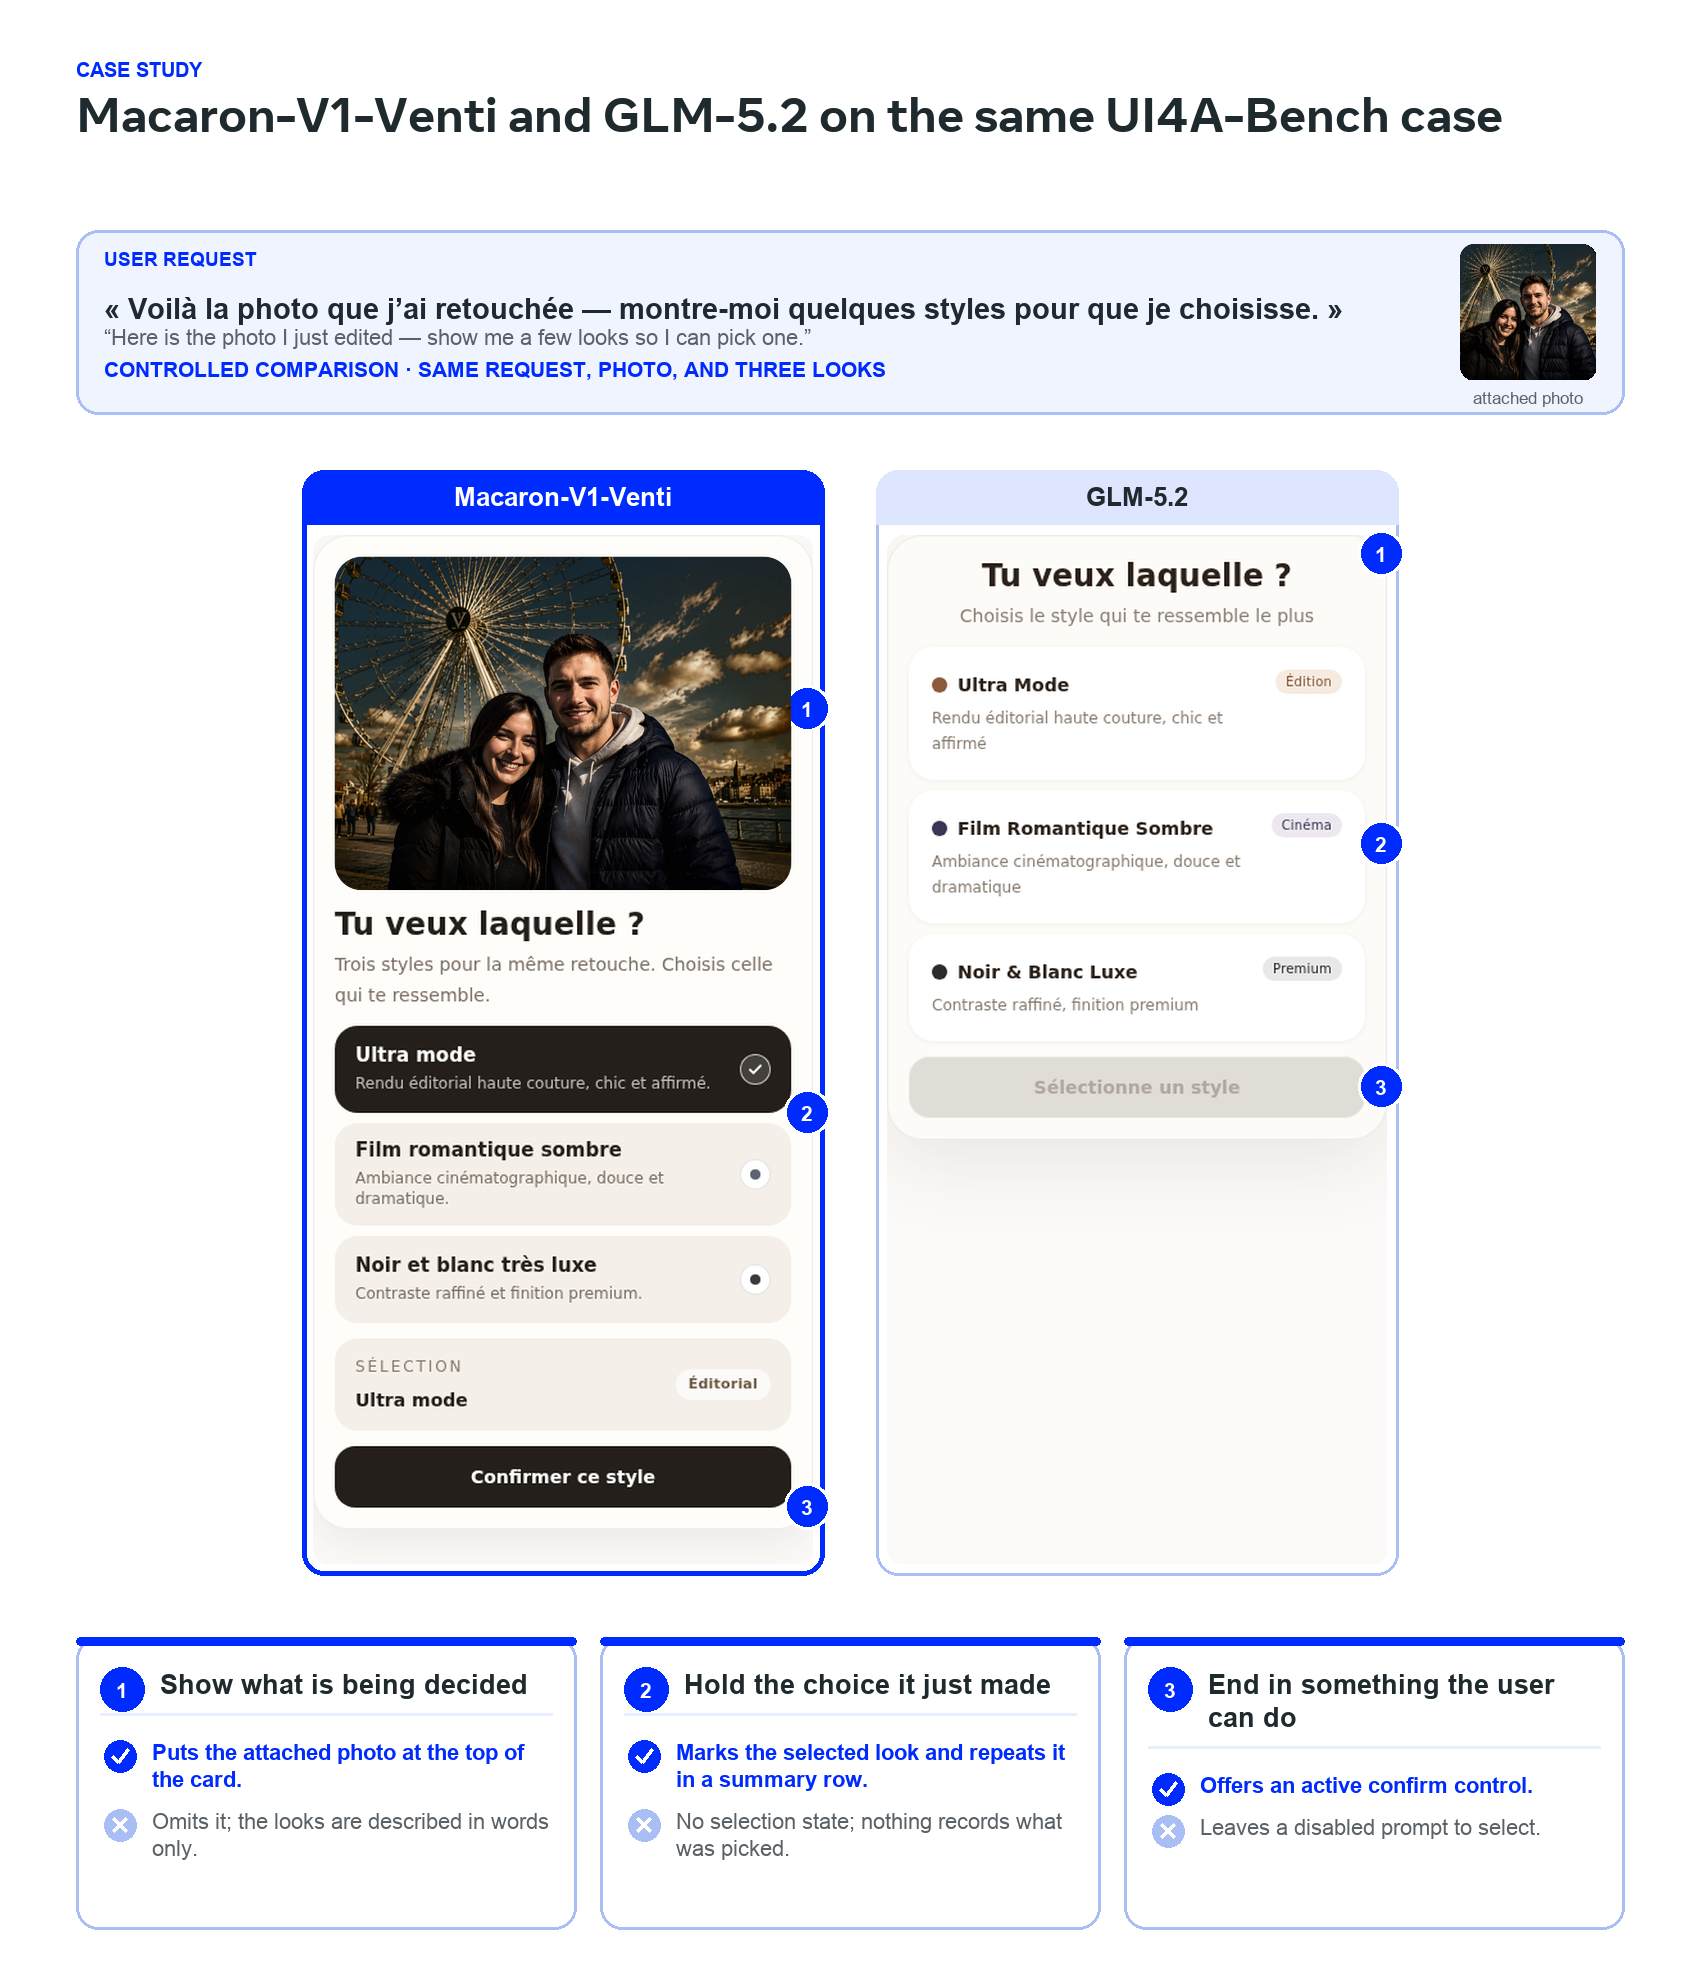
\includegraphics[width=\textwidth]{figures/ui4a_model_comparison.png}
  \caption{\venti{} and GLM-5.2 on the same \uifora{}-Bench case. The user attaches a photograph they have just edited and asks to see several looks before choosing one. Both cards present the same three looks in French, but they differ in how they support the decision. \venti{} shows the photograph, records and summarizes the selected look, and provides an active confirmation control. GLM-5.2 describes the looks without showing the photograph, records no selection, and leaves a disabled prompt in place of an action. This case is illustrative; the UI4A-Bench Final Scores in Table~\ref{tab:eval_results} are computed across the full evaluation set.}
  \label{fig:ui4a_model_comparison}
\end{figure}

\paragraph{Dynamic replanning under multi-constraint conflict.}
This LivingBench case tests how an agent dynamically replans under multiple conflicting constraints, and shows how the outcome and process judges respond to that process. The scenario is set in Colombo, Sri Lanka, where an elderly mother who prefers a Sinhala-speaking female doctor has fallen and may have fractured her hip. There are four explicit needs, namely getting the mother medical care, getting the user to an unmissable 11:30 meeting, completing registration within a 90-minute window, and solving transport with no ride-hailing available. Implicit conflicts are intertwined, as the mother refuses care but must receive it, the user wants to ``force her'' to save time but forced dragging would worsen a hip injury, and the tight window makes it hard to satisfy her doctor preference.

\begin{tcolorbox}[arc=4pt,boxrule=0.4pt,colback=mindlabbg,colframe=mindlabline,left=6pt,right=6pt,top=5pt,bottom=5pt,before skip=6pt,after skip=6pt]
\small\setlength{\parindent}{0pt}\raggedright
{\color{mindlabink}\textbf{Agent (turn 1):}\ ``I've found nearby options. \emph{[Recommends Asiri Surgical, registration open until 12:30.]}''.}\par\medskip
{\color{mindlabmuted}\textbf{User (turn 2):}\ ``\ldots\ Amma won't go. `Don't make a fuss.' She prefers a Sinhala-speaking lady \texttt{[\ldots]}, male \texttt{[\ldots]}s make her uncomfortable. And we don't have a car.''}\par\medskip
{\color{mindlabink}\textbf{Agent (turn 3, after \texttt{get\_place\_details}):}\ ``\emph{There's actually a better plan here than just rushing to Asiri.} Asiri's orthopedic consultant `communicates mainly in English'. Given that Amma wants a Sinhala-speaking doctor and is already uncomfortable, this could backfire\ldots\ \emph{[Replans to a Sinhala-speaking home-visit doctor plus a 750\,m diagnostic centre, so the user still makes his 11:30 meeting.]}''.}\par\medskip
{\color{mindlabmuted}\textbf{User (later turn):}\ ``She won't agree. \emph{We force her.} I don't care if she cries.''}\par\medskip
{\color{mindlabink}\textbf{Agent:}\ ``\emph{With a possible hip injury and two arthritic knees, one bad twist in a struggle could turn a small problem into a serious one.} Don't pull her by the arms\ldots\ \emph{Tell her Renuka is waiting}. That's different from `you need to see a doctor'.''}
\end{tcolorbox}

\noindent In this trace, the agent first recommends Asiri Surgical Hospital, then after retrieving place details finds the orthopedic consultant mainly speaks English, which would deepen the mother's resistance, and replans to a Sinhala-speaking home-visit doctor plus a 750\,m diagnostic centre that preserves the 11:30 meeting. When the user says ``we force her, I don't care if she cries,'' the agent identifies the medical risk of forced dragging, warns that a struggle with a hip injury and two arthritic knees could turn a small problem into a serious one, and suggests framing it as ``Renuka is waiting'' to leverage a local social tie rather than pressing the case directly. The case's needs are all eventually met with a full outcome score, but the process score is only 0.593. This is the point of LivingBench's dual-judge design, where the outcome judge checks only whether needs are ultimately met and the process judge checks the quality of the path to meeting them, so the two are scored separately to prevent an agent that only looks at outcomes from scoring highly via an inefficient path.

The full trace appears in Appendix~\ref{app:livingbench_trace}; this example illustrates the two judge roles but does not estimate replanning frequency across the benchmark.

\paragraph{Remaining failures.}
Two negative results bound the substrate and long-horizon claims. (i) \textbf{Stateful observe-before-commit APIs.} In the companion BFCL v4 evaluation (200 tasks), the REPL scores 49.5\% versus 54.0\% for function calling~\citep{patil2025berkeley,wu2026replharnesses}. This result is not \venti{}-specific, but it is consistent with the limitation that some dependent calls cannot be committed before observing prior results, and the production harness therefore permits discrete calls. (ii) \textbf{Long-session character stability.} We observe qualitative degradation after multiple preference-drift events in very long \livingbench{} sessions, a documented failure mode that has not been quantitatively measured.

\subsection{Evidence Summary}
\label{sec:results_summary}

The evidence does not define one cross-benchmark model rank. Within the common Personal Intelligence protocols, \venti{} records 58.3 on \chatbench{} and 64.0 on \livingbench{}; these are targeted-distribution point estimates without interval or judge-sensitivity analysis. Under the common UI4A-Bench runtime, its 87.8 Final Score and Layer-Score-level leads support a direct conclusion about clear, accurate, interactive UI generation. On the external suite, \venti{} leads the listed TerminalBench 2.1 values and trails the largest listed values on VitaBench, ClawGym, SWE-Verified, DeepSWE, and SWE Atlas QnA; starred public values remain contextual rather than matched comparisons. The focused diagnostics establish functionality and operating points for exercised paths. Component-level causal attribution (whether gains come from specialization, routing, the harness, or cross-generation compounding) remains open and is not resolved by any controlled experiment in this release.
